% SOURCE: ../../edit-harness/results/merging/RG_gain_law_20260715.json + ../../edit-harness/results/merging/RG_admission_benefit_REFIX20260730.json
% !TEX encoding = UTF-8 Unicode
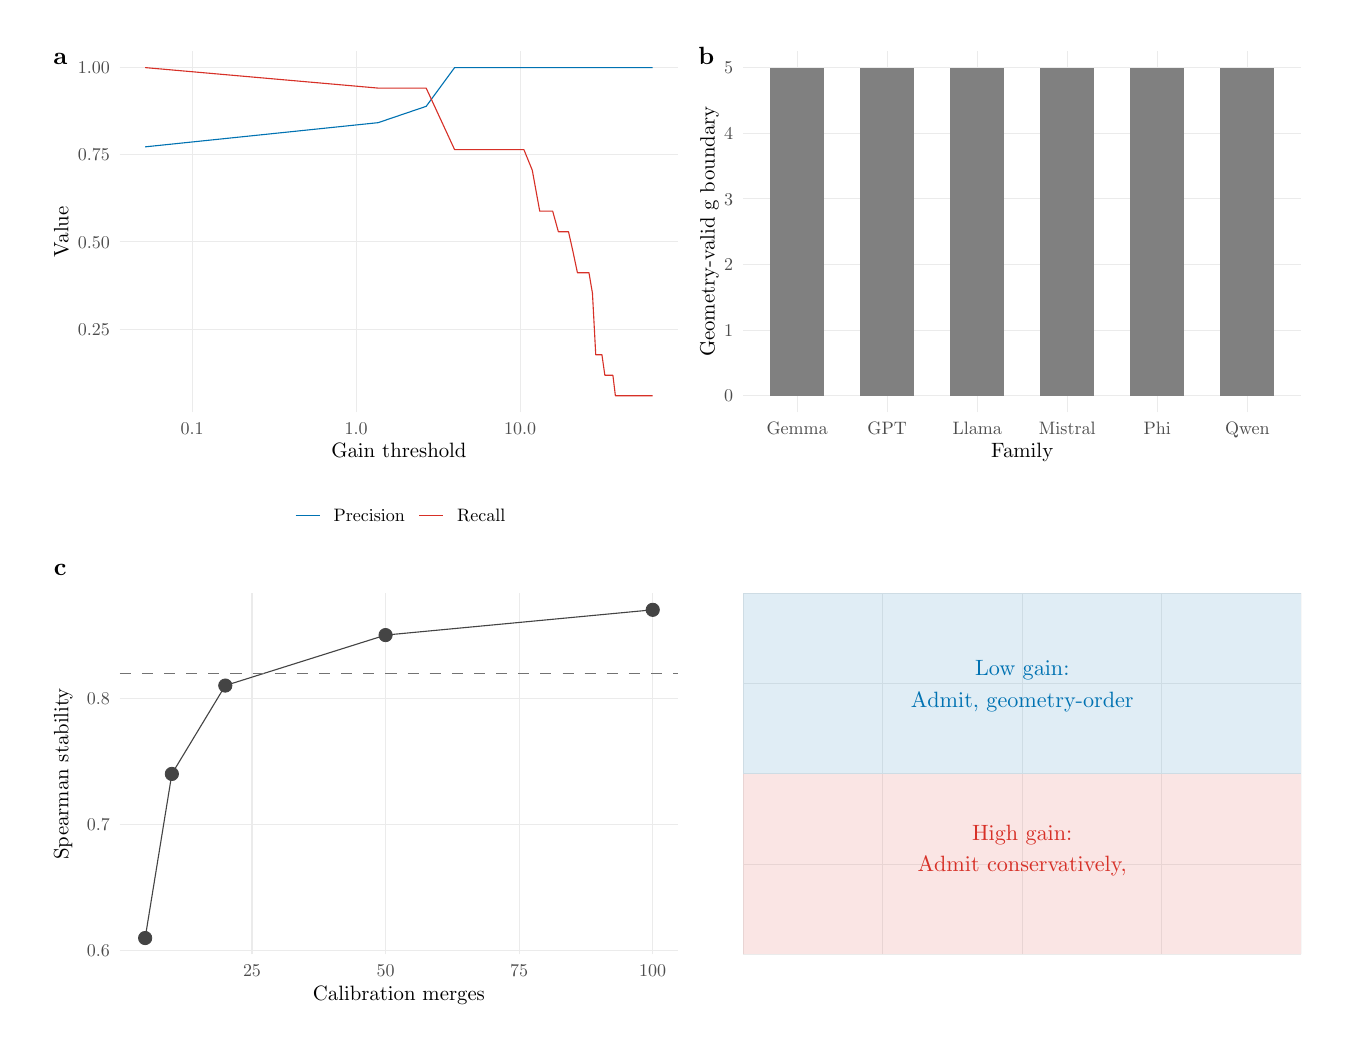
\begin{tikzpicture}[x=1pt,y=1pt]
\definecolor{fillColor}{RGB}{255,255,255}
\path[use as bounding box,fill=fillColor,fill opacity=0.00] (0,0) rectangle (469.75,361.35);
\begin{scope}
\path[clip] (  0.00,  0.00) rectangle (469.75,361.35);
\definecolor{drawColor}{RGB}{255,255,255}
\definecolor{fillColor}{RGB}{255,255,255}

\path[draw=drawColor,line width= 0.6pt,line join=round,line cap=round,fill=fillColor] (  0.00,  0.00) rectangle (469.75,361.35);
\end{scope}
\begin{scope}
\path[clip] (  5.50,170.98) rectangle (239.03,355.85);
\definecolor{fillColor}{RGB}{255,255,255}

\path[fill=fillColor] (  5.50,170.98) rectangle (239.03,355.85);
\end{scope}
\begin{scope}
\path[clip] (239.03,170.98) rectangle (464.25,355.85);
\definecolor{fillColor}{RGB}{255,255,255}

\path[fill=fillColor] (239.03,170.98) rectangle (464.25,355.85);
\end{scope}
\begin{scope}
\path[clip] (  5.50,  5.50) rectangle (239.03,170.98);
\definecolor{fillColor}{RGB}{255,255,255}

\path[fill=fillColor] (  5.50,  5.50) rectangle (239.03,170.98);
\end{scope}
\begin{scope}
\path[clip] (239.03,  5.50) rectangle (464.25,170.98);
\definecolor{fillColor}{RGB}{255,255,255}

\path[fill=fillColor] (239.03,  5.50) rectangle (464.25,170.98);
\end{scope}
\begin{scope}
\path[clip] ( 33.28,222.40) rectangle (235.03,352.85);
\definecolor{drawColor}{gray}{0.92}

\path[draw=drawColor,line width= 0.4pt,line join=round] ( 33.28,252.42) --
	(235.03,252.42);

\path[draw=drawColor,line width= 0.4pt,line join=round] ( 33.28,283.92) --
	(235.03,283.92);

\path[draw=drawColor,line width= 0.4pt,line join=round] ( 33.28,315.42) --
	(235.03,315.42);

\path[draw=drawColor,line width= 0.4pt,line join=round] ( 33.28,346.92) --
	(235.03,346.92);

\path[draw=drawColor,line width= 0.4pt,line join=round] ( 59.40,222.40) --
	( 59.40,352.85);

\path[draw=drawColor,line width= 0.4pt,line join=round] (118.68,222.40) --
	(118.68,352.85);

\path[draw=drawColor,line width= 0.4pt,line join=round] (177.95,222.40) --
	(177.95,352.85);
\definecolor{drawColor}{RGB}{0,114,178}

\path[draw=drawColor,line width= 0.4pt,line join=round] ( 42.45,318.28) --
	(126.65,327.02) --
	(144.00,332.92) --
	(154.27,346.92) --
	(161.59,346.92) --
	(167.29,346.92) --
	(171.95,346.92) --
	(175.89,346.92) --
	(179.31,346.92) --
	(182.33,346.92) --
	(185.03,346.92) --
	(187.47,346.92) --
	(189.71,346.92) --
	(191.76,346.92) --
	(193.66,346.92) --
	(195.43,346.92) --
	(197.09,346.92) --
	(198.65,346.92) --
	(200.12,346.92) --
	(201.50,346.92) --
	(202.82,346.92) --
	(204.08,346.92) --
	(205.27,346.92) --
	(206.41,346.92) --
	(207.51,346.92) --
	(208.56,346.92) --
	(209.56,346.92) --
	(210.53,346.92) --
	(211.47,346.92) --
	(212.37,346.92) --
	(213.24,346.92) --
	(214.09,346.92) --
	(214.90,346.92) --
	(215.69,346.92) --
	(216.46,346.92) --
	(217.21,346.92) --
	(217.93,346.92) --
	(218.63,346.92) --
	(219.32,346.92) --
	(219.99,346.92) --
	(220.64,346.92) --
	(221.27,346.92) --
	(221.89,346.92) --
	(222.50,346.92) --
	(223.09,346.92) --
	(223.67,346.92) --
	(224.23,346.92) --
	(224.79,346.92) --
	(225.33,346.92) --
	(225.86,346.92);
\definecolor{drawColor}{RGB}{215,48,39}

\path[draw=drawColor,line width= 0.4pt,line join=round] ( 42.45,346.92) --
	(126.65,339.51) --
	(144.00,339.51) --
	(154.27,317.27) --
	(161.59,317.27) --
	(167.29,317.27) --
	(171.95,317.27) --
	(175.89,317.27) --
	(179.31,317.27) --
	(182.33,309.86) --
	(185.03,295.04) --
	(187.47,295.04) --
	(189.71,295.04) --
	(191.76,287.62) --
	(193.66,287.62) --
	(195.43,287.62) --
	(197.09,280.21) --
	(198.65,272.80) --
	(200.12,272.80) --
	(201.50,272.80) --
	(202.82,272.80) --
	(204.08,265.39) --
	(205.27,243.15) --
	(206.41,243.15) --
	(207.51,243.15) --
	(208.56,235.74) --
	(209.56,235.74) --
	(210.53,235.74) --
	(211.47,235.74) --
	(212.37,228.33) --
	(213.24,228.33) --
	(214.09,228.33) --
	(214.90,228.33) --
	(215.69,228.33) --
	(216.46,228.33) --
	(217.21,228.33) --
	(217.93,228.33) --
	(218.63,228.33) --
	(219.32,228.33) --
	(219.99,228.33) --
	(220.64,228.33) --
	(221.27,228.33) --
	(221.89,228.33) --
	(222.50,228.33) --
	(223.09,228.33) --
	(223.67,228.33) --
	(224.23,228.33) --
	(224.79,228.33) --
	(225.33,228.33) --
	(225.86,228.33);
\end{scope}
\begin{scope}
\path[clip] (  0.00,  0.00) rectangle (469.75,361.35);
\definecolor{drawColor}{gray}{0.30}

\node[text=drawColor,anchor=base east,inner sep=0pt, outer sep=0pt, scale=  0.65] at ( 29.68,250.18) {0.25};

\node[text=drawColor,anchor=base east,inner sep=0pt, outer sep=0pt, scale=  0.65] at ( 29.68,281.68) {0.50};

\node[text=drawColor,anchor=base east,inner sep=0pt, outer sep=0pt, scale=  0.65] at ( 29.68,313.18) {0.75};

\node[text=drawColor,anchor=base east,inner sep=0pt, outer sep=0pt, scale=  0.65] at ( 29.68,344.68) {1.00};
\end{scope}
\begin{scope}
\path[clip] (  0.00,  0.00) rectangle (469.75,361.35);
\definecolor{drawColor}{gray}{0.30}

\node[text=drawColor,anchor=base,inner sep=0pt, outer sep=0pt, scale=  0.65] at ( 59.40,214.32) {0.1};

\node[text=drawColor,anchor=base,inner sep=0pt, outer sep=0pt, scale=  0.65] at (118.68,214.32) {1.0};

\node[text=drawColor,anchor=base,inner sep=0pt, outer sep=0pt, scale=  0.65] at (177.95,214.32) {10.0};
\end{scope}
\begin{scope}
\path[clip] (  0.00,  0.00) rectangle (469.75,361.35);
\definecolor{drawColor}{RGB}{0,0,0}

\node[text=drawColor,anchor=base,inner sep=0pt, outer sep=0pt, scale=  0.75] at (134.15,205.89) {Gain threshold};
\end{scope}
\begin{scope}
\path[clip] (  0.00,  0.00) rectangle (469.75,361.35);
\definecolor{drawColor}{RGB}{0,0,0}

\node[text=drawColor,rotate= 90.00,anchor=base,inner sep=0pt, outer sep=0pt, scale=  0.75] at ( 14.67,287.62) {Value};
\end{scope}
\begin{scope}
\path[clip] (  0.00,  0.00) rectangle (469.75,361.35);
\definecolor{drawColor}{RGB}{0,114,178}

\path[draw=drawColor,line width= 0.4pt,line join=round] ( 96.80,185.21) -- (105.47,185.21);
\end{scope}
\begin{scope}
\path[clip] (  0.00,  0.00) rectangle (469.75,361.35);
\definecolor{drawColor}{RGB}{215,48,39}

\path[draw=drawColor,line width= 0.4pt,line join=round] (141.42,185.21) -- (150.09,185.21);
\end{scope}
\begin{scope}
\path[clip] (  0.00,  0.00) rectangle (469.75,361.35);
\definecolor{drawColor}{RGB}{0,0,0}

\node[text=drawColor,anchor=base west,inner sep=0pt, outer sep=0pt, scale=  0.65] at (110.55,182.97) {Precision};
\end{scope}
\begin{scope}
\path[clip] (  0.00,  0.00) rectangle (469.75,361.35);
\definecolor{drawColor}{RGB}{0,0,0}

\node[text=drawColor,anchor=base west,inner sep=0pt, outer sep=0pt, scale=  0.65] at (155.17,182.97) {Recall};
\end{scope}
\begin{scope}
\path[clip] (  0.00,  0.00) rectangle (469.75,361.35);
\definecolor{drawColor}{RGB}{0,0,0}

\node[text=drawColor,anchor=base,inner sep=0pt, outer sep=0pt, scale=  0.90] at ( 11.76,347.96) {\bfseries a};
\end{scope}
\begin{scope}
\path[clip] (258.50,222.40) rectangle (460.25,352.85);
\definecolor{drawColor}{gray}{0.92}

\path[draw=drawColor,line width= 0.4pt,line join=round] (258.50,228.33) --
	(460.25,228.33);

\path[draw=drawColor,line width= 0.4pt,line join=round] (258.50,252.05) --
	(460.25,252.05);

\path[draw=drawColor,line width= 0.4pt,line join=round] (258.50,275.76) --
	(460.25,275.76);

\path[draw=drawColor,line width= 0.4pt,line join=round] (258.50,299.48) --
	(460.25,299.48);

\path[draw=drawColor,line width= 0.4pt,line join=round] (258.50,323.20) --
	(460.25,323.20);

\path[draw=drawColor,line width= 0.4pt,line join=round] (258.50,346.92) --
	(460.25,346.92);

\path[draw=drawColor,line width= 0.4pt,line join=round] (278.03,222.40) --
	(278.03,352.85);

\path[draw=drawColor,line width= 0.4pt,line join=round] (310.57,222.40) --
	(310.57,352.85);

\path[draw=drawColor,line width= 0.4pt,line join=round] (343.11,222.40) --
	(343.11,352.85);

\path[draw=drawColor,line width= 0.4pt,line join=round] (375.65,222.40) --
	(375.65,352.85);

\path[draw=drawColor,line width= 0.4pt,line join=round] (408.19,222.40) --
	(408.19,352.85);

\path[draw=drawColor,line width= 0.4pt,line join=round] (440.73,222.40) --
	(440.73,352.85);
\definecolor{fillColor}{gray}{0.50}

\path[fill=fillColor] (333.35,228.33) rectangle (352.87,346.92);

\path[fill=fillColor] (430.97,228.33) rectangle (450.49,346.92);

\path[fill=fillColor] (398.43,228.33) rectangle (417.95,346.92);

\path[fill=fillColor] (268.26,228.33) rectangle (287.79,346.92);

\path[fill=fillColor] (300.80,228.33) rectangle (320.33,346.92);

\path[fill=fillColor] (365.89,228.33) rectangle (385.41,346.92);
\end{scope}
\begin{scope}
\path[clip] (  0.00,  0.00) rectangle (469.75,361.35);
\definecolor{drawColor}{gray}{0.30}

\node[text=drawColor,anchor=base east,inner sep=0pt, outer sep=0pt, scale=  0.65] at (254.90,226.09) {0};

\node[text=drawColor,anchor=base east,inner sep=0pt, outer sep=0pt, scale=  0.65] at (254.90,249.81) {1};

\node[text=drawColor,anchor=base east,inner sep=0pt, outer sep=0pt, scale=  0.65] at (254.90,273.53) {2};

\node[text=drawColor,anchor=base east,inner sep=0pt, outer sep=0pt, scale=  0.65] at (254.90,297.24) {3};

\node[text=drawColor,anchor=base east,inner sep=0pt, outer sep=0pt, scale=  0.65] at (254.90,320.96) {4};

\node[text=drawColor,anchor=base east,inner sep=0pt, outer sep=0pt, scale=  0.65] at (254.90,344.68) {5};
\end{scope}
\begin{scope}
\path[clip] (  0.00,  0.00) rectangle (469.75,361.35);
\definecolor{drawColor}{gray}{0.30}

\node[text=drawColor,anchor=base,inner sep=0pt, outer sep=0pt, scale=  0.65] at (278.03,214.32) {Gemma};

\node[text=drawColor,anchor=base,inner sep=0pt, outer sep=0pt, scale=  0.65] at (310.57,214.32) {GPT};

\node[text=drawColor,anchor=base,inner sep=0pt, outer sep=0pt, scale=  0.65] at (343.11,214.32) {Llama};

\node[text=drawColor,anchor=base,inner sep=0pt, outer sep=0pt, scale=  0.65] at (375.65,214.32) {Mistral};

\node[text=drawColor,anchor=base,inner sep=0pt, outer sep=0pt, scale=  0.65] at (408.19,214.32) {Phi};

\node[text=drawColor,anchor=base,inner sep=0pt, outer sep=0pt, scale=  0.65] at (440.73,214.32) {Qwen};
\end{scope}
\begin{scope}
\path[clip] (  0.00,  0.00) rectangle (469.75,361.35);
\definecolor{drawColor}{RGB}{0,0,0}

\node[text=drawColor,anchor=base,inner sep=0pt, outer sep=0pt, scale=  0.75] at (359.38,205.89) {Family};
\end{scope}
\begin{scope}
\path[clip] (  0.00,  0.00) rectangle (469.75,361.35);
\definecolor{drawColor}{RGB}{0,0,0}

\node[text=drawColor,rotate= 90.00,anchor=base,inner sep=0pt, outer sep=0pt, scale=  0.75] at (248.19,287.62) {Geometry-valid g boundary};
\end{scope}
\begin{scope}
\path[clip] (  0.00,  0.00) rectangle (469.75,361.35);
\definecolor{drawColor}{RGB}{0,0,0}

\node[text=drawColor,anchor=base,inner sep=0pt, outer sep=0pt, scale=  0.90] at (245.20,347.96) {\bfseries b};
\end{scope}
\begin{scope}
\path[clip] ( 33.28, 26.46) rectangle (235.03,156.92);
\definecolor{drawColor}{gray}{0.92}

\path[draw=drawColor,line width= 0.4pt,line join=round] ( 33.28, 27.83) --
	(235.03, 27.83);

\path[draw=drawColor,line width= 0.4pt,line join=round] ( 33.28, 73.44) --
	(235.03, 73.44);

\path[draw=drawColor,line width= 0.4pt,line join=round] ( 33.28,119.06) --
	(235.03,119.06);

\path[draw=drawColor,line width= 0.4pt,line join=round] ( 81.06, 26.46) --
	( 81.06,156.92);

\path[draw=drawColor,line width= 0.4pt,line join=round] (129.33, 26.46) --
	(129.33,156.92);

\path[draw=drawColor,line width= 0.4pt,line join=round] (177.59, 26.46) --
	(177.59,156.92);

\path[draw=drawColor,line width= 0.4pt,line join=round] (225.86, 26.46) --
	(225.86,156.92);
\definecolor{drawColor}{RGB}{68,68,68}

\path[draw=drawColor,line width= 0.4pt,line join=round] ( 42.45, 32.39) --
	( 52.10, 91.69) --
	( 71.41,123.62) --
	(129.33,141.86) --
	(225.86,150.99);
\definecolor{fillColor}{RGB}{68,68,68}

\path[draw=drawColor,line width= 0.3pt,line join=round,line cap=round,fill=fillColor] ( 42.45, 32.39) circle (  2.40);

\path[draw=drawColor,line width= 0.3pt,line join=round,line cap=round,fill=fillColor] ( 52.10, 91.69) circle (  2.40);

\path[draw=drawColor,line width= 0.3pt,line join=round,line cap=round,fill=fillColor] ( 71.41,123.62) circle (  2.40);

\path[draw=drawColor,line width= 0.3pt,line join=round,line cap=round,fill=fillColor] (129.33,141.86) circle (  2.40);

\path[draw=drawColor,line width= 0.3pt,line join=round,line cap=round,fill=fillColor] (225.86,150.99) circle (  2.40);
\definecolor{drawColor}{gray}{0.45}

\path[draw=drawColor,line width= 0.3pt,dash pattern=on 4pt off 4pt ,line join=round] ( 33.28,128.18) -- (235.03,128.18);
\end{scope}
\begin{scope}
\path[clip] (  0.00,  0.00) rectangle (469.75,361.35);
\definecolor{drawColor}{gray}{0.30}

\node[text=drawColor,anchor=base east,inner sep=0pt, outer sep=0pt, scale=  0.65] at ( 29.68, 25.59) {0.6};

\node[text=drawColor,anchor=base east,inner sep=0pt, outer sep=0pt, scale=  0.65] at ( 29.68, 71.21) {0.7};

\node[text=drawColor,anchor=base east,inner sep=0pt, outer sep=0pt, scale=  0.65] at ( 29.68,116.82) {0.8};
\end{scope}
\begin{scope}
\path[clip] (  0.00,  0.00) rectangle (469.75,361.35);
\definecolor{drawColor}{gray}{0.30}

\node[text=drawColor,anchor=base,inner sep=0pt, outer sep=0pt, scale=  0.65] at ( 81.06, 18.39) {25};

\node[text=drawColor,anchor=base,inner sep=0pt, outer sep=0pt, scale=  0.65] at (129.33, 18.39) {50};

\node[text=drawColor,anchor=base,inner sep=0pt, outer sep=0pt, scale=  0.65] at (177.59, 18.39) {75};

\node[text=drawColor,anchor=base,inner sep=0pt, outer sep=0pt, scale=  0.65] at (225.86, 18.39) {100};
\end{scope}
\begin{scope}
\path[clip] (  0.00,  0.00) rectangle (469.75,361.35);
\definecolor{drawColor}{RGB}{0,0,0}

\node[text=drawColor,anchor=base,inner sep=0pt, outer sep=0pt, scale=  0.75] at (134.15,  9.96) {Calibration merges};
\end{scope}
\begin{scope}
\path[clip] (  0.00,  0.00) rectangle (469.75,361.35);
\definecolor{drawColor}{RGB}{0,0,0}

\node[text=drawColor,rotate= 90.00,anchor=base,inner sep=0pt, outer sep=0pt, scale=  0.75] at ( 14.67, 91.69) {Spearman stability};
\end{scope}
\begin{scope}
\path[clip] (  0.00,  0.00) rectangle (469.75,361.35);
\definecolor{drawColor}{RGB}{0,0,0}

\node[text=drawColor,anchor=base,inner sep=0pt, outer sep=0pt, scale=  0.90] at ( 11.76,163.28) {\bfseries c};
\end{scope}
\begin{scope}
\path[clip] (258.50, 26.46) rectangle (460.25,156.92);
\definecolor{drawColor}{gray}{0.92}

\path[draw=drawColor,line width= 0.4pt,line join=round] (258.50, 26.46) --
	(460.25, 26.46);

\path[draw=drawColor,line width= 0.4pt,line join=round] (258.50, 59.08) --
	(460.25, 59.08);

\path[draw=drawColor,line width= 0.4pt,line join=round] (258.50, 91.69) --
	(460.25, 91.69);

\path[draw=drawColor,line width= 0.4pt,line join=round] (258.50,124.30) --
	(460.25,124.30);

\path[draw=drawColor,line width= 0.4pt,line join=round] (258.50,156.92) --
	(460.25,156.92);

\path[draw=drawColor,line width= 0.4pt,line join=round] (258.50, 26.46) --
	(258.50,156.92);

\path[draw=drawColor,line width= 0.4pt,line join=round] (308.94, 26.46) --
	(308.94,156.92);

\path[draw=drawColor,line width= 0.4pt,line join=round] (359.38, 26.46) --
	(359.38,156.92);

\path[draw=drawColor,line width= 0.4pt,line join=round] (409.82, 26.46) --
	(409.82,156.92);

\path[draw=drawColor,line width= 0.4pt,line join=round] (460.25, 26.46) --
	(460.25,156.92);
\definecolor{fillColor}{RGB}{0,114,178}

\path[fill=fillColor,fill opacity=0.12] (258.50, 91.69) rectangle (460.25,156.92);
\definecolor{fillColor}{RGB}{215,48,39}

\path[fill=fillColor,fill opacity=0.12] (258.50, 26.46) rectangle (460.25, 91.69);
\definecolor{drawColor}{RGB}{0,114,178}

\node[text=drawColor,anchor=base,inner sep=0pt, outer sep=0pt, scale=  0.80] at (359.38,127.30) {Low gain:};

\node[text=drawColor,anchor=base,inner sep=0pt, outer sep=0pt, scale=  0.80] at (359.38,115.82) {Admit, geometry-order};
\definecolor{drawColor}{RGB}{215,48,39}

\node[text=drawColor,anchor=base,inner sep=0pt, outer sep=0pt, scale=  0.80] at (359.38, 67.81) {High gain:};

\node[text=drawColor,anchor=base,inner sep=0pt, outer sep=0pt, scale=  0.80] at (359.38, 56.33) {Admit conservatively,};
\end{scope}
\end{tikzpicture}
